\documentclass[
	12pt,            % Tamanho da fonte
	oneside,         % Para impressão em uma face
	a4paper,         % Tamanho do papel A4
	english,         % Idioma secundário
	brazil           % Idioma principal
]{abntex2}

\usepackage{graphicx}          % Para incluir imagens
\usepackage[utf8]{inputenc}    % Codificação UTF-8
\usepackage[T1]{fontenc}       % Encoding para fontes
\usepackage{indentfirst}       % Indenta o primeiro parágrafo de cada seção
\usepackage{microtype}         % Melhorias na justificação do texto
\usepackage{hyperref}          % Links clicáveis
\usepackage{amsmath,amssymb}   % Pacotes matemáticos
\usepackage{wasysym}           % Para símbolos incluindo checkbox
\usepackage{setspace}
\usepackage{float}             % Controle preciso de posicionamento de floats
\usepackage{xcolor}

% Configurações de margens
\usepackage{geometry}
\usepackage{tabularx} % Coloque isso no preâmbulo

\geometry{
	a4paper,
	left=3cm,        % Margem esquerda
	right=2cm,       % Margem direita
	top=3cm,         % Margem superior
	bottom=2cm       % Margem inferior
}

\setlength{\parindent}{1.25cm}  % Recuo da primeira linha do parágrafo
\setlength{\parskip}{0.2cm}     % Espaço entre parágrafos

\title{Análise de Crescimento de Plantas a Partir de Fotos Semanais}
\author{
    Lucas Cardoso dos Santos \\
    Lucas Miranda Mendonça Rezende
}
\date{Ribeirão Preto\\2025}

\begin{document}

\begin{center} 
    Universidade de São Paulo \linebreak
    Faculdade de Filosofia, Ciências e Letras de Ribeirão Preto (FFCLRP) \linebreak
    Departamento de Computação e Matemática (DCM)
    
    \vfill
    
    \Large Processamento de Imagens % TÍTULO
    
    \Huge Plant Growth: Análise de Crescimento de Plantas a Partir de Fotos Semanais % TÍTULO
    
    \normalsize
    \vfill
    
    % NOMES
    Lucas Cardoso dos Santos (9865492)

    Lucas Miranda Mendonça Rezende (12542838)

    \vfill
    
    Ribeirão Preto
    
    2025
    
\end{center} %página1%

\newpage
\tableofcontents

\chapter*{Resumo}
 
No cenário agrícola atual de pressão por maior produtividade e uso racional de recursos, a Agricultura Inteligente surge como ponte entre tecnologia e sustentabilidade. Neste trabalho, propomos um método automatizado de extração de métricas de crescimento de plantas (área, altura e largura) a partir de imagens digitais. A metodologia combina segmentação com análise geométrica. O sistema demonstra capacidade de gerar indicadores confiáveis para monitoramento contínuo em diferentes tipos de imagens, permitindo detecção de estresses bióticos e abióticos, planejamento de irrigação e insumos, além de servir de base para benchmarks de produtividade. Desenvolvida como uma interface intuitiva, a solução facilita o acesso de produtores e pesquisadores a dados objetivos, promovendo decisões mais informadas na agricultura.

\chapter{Introdução}

A Agricultura Inteligente é a aplicação de tecnologias avançadas ao setor agrícola, com o objetivo de tornar as práticas de cultivo mais eficientes e sustentáveis. Alguns casos práticos de aplicação desses sistemas são sistemas de gerenciamento de irrigação, uso controlado de fertilizantes, e monitoramento da qualidade da plantação. O uso de câmeras na agricultura inteligente é cada vez mais comum e, com isso, inúmeras novas possibilidades são permitidas no controle e acompanhamento da produção.

A obtenção de dados é um dos cernes da agricultura inteligente. Como tal, precisamos de meios de qualificar e quantificar as melhorias obtidas com uso de ferramentas novas, técnicas mais avançadas e recursos diferentes. Visando criar e aprimorar métodos existentes de análise das plantações, os autores propõem um método eficiente de base para, a partir de imagens relativamente complexas para processamento, obter a área, a altura e a largura das plantas representadas, de modo que seja possível acompanhar e avaliar o crescimento destas. 

As aplicações deste método, porém, vão consideravelmente além deste escopo: criação de benchmarks para avaliar cientificamente o desenvolvimento, quantificar a estimativa de retorno de safras agrícolas, monitorar a saúde das culturas em tempo real, detectar precocemente sinais de pragas ou doenças, otimizar o uso de recursos como água e fertilizantes, planejar a logística de colheitas de forma mais eficiente, e apoiar decisões estratégicas de manejo agrícola com base em dados concretos.

\chapter{Materiais e Métodos}

Para a solução do problema de acompanhamento do crescimento de plantas, principalmente em contextos de larga escala, como grandes fazendas, os autores propõem aqui uma solução que se baseia na segmentação das imagens obtidas e extração de medidas a partir do segmento correspondente à planta.

Existem diversos algoritmos para segmentar a imagem e obter corretamente os pixels correspondentes à planta. Estratégias mais simples como a definição de um limiar para os valores aceitáveis de verde, por exemplo, podem ser aplicadas, embora sua simplicidade (e, portanto, facilidade de implementação) resulte em resultados menos adequados. Também existem técnicas mais avançadas e robustas, como o uso de algoritmos de aprendizado de máquina, cabendo aos autores fazer o treinamento desses algoritmos para obter os resultados com a precisão que desejamos. Durante a execução desse trabalho, os autores pretendem determinar qual estratégia de segmentação é a mais apropriada para os resultados desejados.

A extração de medidas, assumindo um algoritmo perfeito de segmentação, torna-se elementar. Para obter os dados da área precisamos apenas contar os pixels que existem naquele segmento. Para altura da planta, a estratégia escolhida é realizar uma regressão linear com os pontos do segmento, assim normalizando a possivel rotação da imagem, a partir do sistema de coordenadas baseado na reta obtida podemos obter os pontos máximo e mínimo no eixo Y, que correspondem à altura. Para a largura, projetamos os pontos do segmento no eixo X deste sistema de coordenadas e obtemos a distância entre os pontos máximo e mínimo, que correspondem à largura da planta.

Quanto aos materiais necessários, estes consistem simplesmente de imagens de plantas. Qualquer imagem encontrada na internet que mostre uma planta pode ser utilizada para testar a aplicação final. Além disso, pode-se fazer necessário o uso de um \textit{dataset} de imagens para o treinamento do algoritmo de aprendizado de máquina, caso esta seja a estratégia de segmentação adotada. Este deve ser composto por imagens de plantas com a segmentação já feita. Existem diversos \textit{datasets} disponíveis na internet que podem ser utilizados para esse fim.

Quanto a limitações, espera-se que, dependendo do algoritmo de segmentação escolhido, a imagem pode não ser segmentada corretamente caso existam outros elementos de cor semelhante ao verde. Outra limitação dá-se pela natureza do algoritmo de regressão linear, que dependendo da orientação da planta (mais horizontal ou vertical) pode inverter logicamente os valores de altura e largura, embora na imagem final isso seja representado de forma indiferente. Também é importante ressaltar que foge do escopo deste trabalho a conversão de medidas de pixels para medidas reais, como centímetros ou metros, uma vez que isso depende de diversos fatores como a distância da câmera em relação à planta, a qualidade da imagem, entre outros. Dado isso, para que as medidas sejam consistentes no tempo, é importante que as imagens sejam tiradas sempre da mesma distância, ângulo e condições de iluminação.

A aplicação final deve então utilizar esses algoritmos de segmentação, determinação de área, altura e largura para entregar ao usuário uma interface onde ele pode enviar as imagens de suas plantas, obtendo assim a imagem processada, composta pela imagem original com uma máscara aplicada e os dados de área, altura e largura da planta, como observado na Figura \ref{fig:exemplo-imagem-processada}.

\begin{figure}
    \centering
    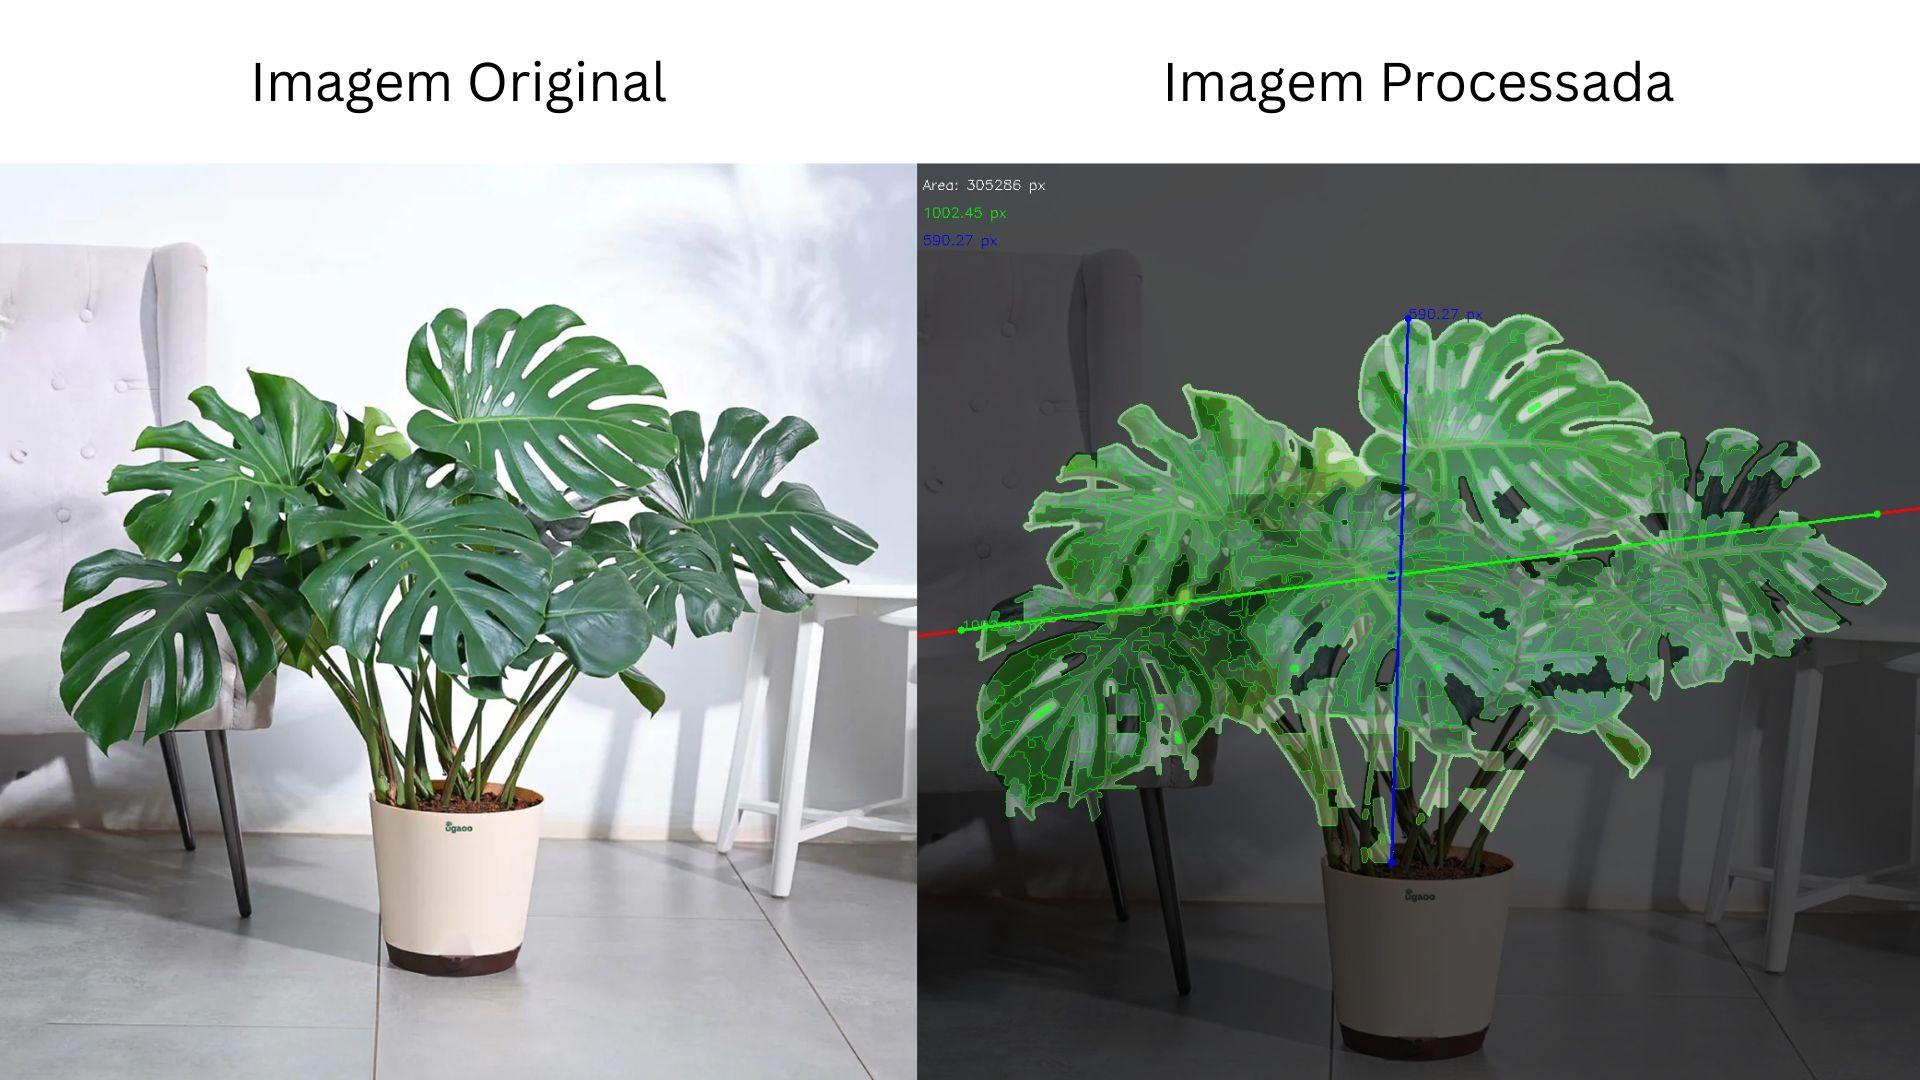
\includegraphics[width=1\textwidth]{../figures/pi/exemplo-imagem-processada.jpg}
    \caption{Imagem processada com a máscara aplicada e os dados de área, altura e largura da planta. Fonte: os autores.}
    \label{fig:exemplo-imagem-processada}
\end{figure}

\chapter{Desenvolvimento do Sistema}

\section{Visão Geral do Projeto}

A aplicação desenvolvida tem como objetivo principal automatizar a quantificação do crescimento de plantas a partir de imagens digitais, proporcionando uma ferramenta acessível para pesquisadores, agrônomos e demais interessados. Por meio do processamento automatizado de fotos, o sistema permite extrair medidas morfológicas relevantes (área, altura e largura) de plantas ao longo do tempo, facilitando o acompanhamento do desenvolvimento vegetal em experimentos ou cultivos. A interface gráfica foi projetada para tornar o processo intuitivo, desde a organização das imagens em coleções até a visualização dos resultados e geração de gráficos de crescimento, promovendo eficiência na análise de dados.

\begin{figure}[H]
    \centering
    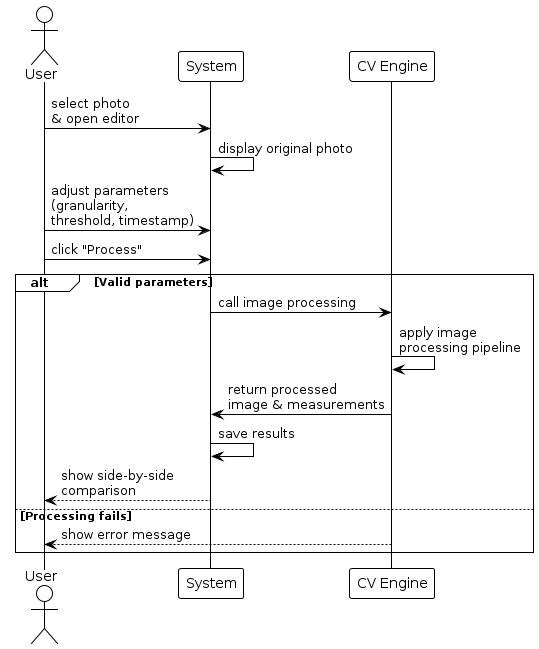
\includegraphics[width=0.45\textwidth]{../figures/dss/UC011.png}
    \caption{Diagrama de sequência do processamento de uma foto individual. Fonte: os autores}
    \label{fig:uc011-process-single-photo}
\end{figure}

\subsection{Processamento de Imagem}

A quantificação do crescimento de plantas a partir de imagens envolve uma série de conceitos fundamentais de processamento de imagem, com destaque para segmentação, análise de cor e extração de medidas morfológicas. O primeiro desafio é separar a planta do fundo da imagem, tarefa conhecida como segmentação.

Para isso, utilizamos o algoritmo watershed. O algoritmo interpreta a imagem em tons de cinza como uma superfície topográfica, onde os valores de intensidade representam elevações. Inicialmente, marcadores são definidos em regiões de interesse (como fundo e possíveis objetos). A partir desses marcadores, o algoritmo simula o preenchimento dessas regiões com "água". À medida que a água se espalha, ela encontra barreiras naturais (bordas) e, quando duas regiões em expansão se encontram, uma linha de separação é criada, formando as fronteiras entre os objetos segmentados. Esse processo resulta em uma segmentação precisa, especialmente útil para separar objetos conectados ou com contornos pouco definidos.

Após a segmentação, é necessário identificar qual das regiões corresponde de fato à planta. Para isso, analisamos as propriedades de cor das regiões segmentadas, utilizando tanto o modelo tradicional RGB (ou BGR) quanto o modelo HSV, que separa matiz, saturação e valor. A predominância de tons de verde é o principal critério para reconhecer a área foliar, já que a maioria das plantas apresenta essa característica. O uso combinado de diferentes espaços de cor torna o processo mais robusto a variações de iluminação e tonalidade.

Com a planta isolada, aplicam-se operações morfológicas para corrigir pequenas falhas na máscara, como buracos ou regiões desconectadas, garantindo que a área da planta seja representada de forma contínua. A partir dessa máscara, extraímos medidas morfológicas relevantes: a área, dada pela contagem de pixels; a altura, que corresponde à maior extensão da planta ao longo de seu eixo principal, obtida por regressão linear dos pontos segmentados; e a largura, medida perpendicularmente à altura. Essas medidas permitem acompanhar o desenvolvimento da planta ao longo do tempo de maneira objetiva e automatizada.

Por fim, a visualização dos resultados é facilitada pela sobreposição da máscara segmentada e das linhas de medição sobre a imagem original, tornando o processo interpretável e útil para o usuário.

\subsection{Interface Gráfica}

A interface gráfica da aplicação oferece um conjunto de funcionalidades que tornam o acompanhamento do crescimento de plantas prático e eficiente. O usuário pode criar coleções para organizar fotos de uma mesma planta ou experimento ao longo do tempo, facilitando o gerenciamento e a comparação dos resultados. É possível associar ou desassociar fotos de uma coleção, renomear ou excluir coleções inteiras, e visualizar todas as imagens agrupadas de forma estruturada.

Além disso, a interface permite o envio e processamento de fotos individuais ou múltiplas de uma só vez, tornando simples tanto testes rápidos quanto o acompanhamento de experimentos. Após o processamento, o usuário pode visualizar as imagens segmentadas com as medidas extraídas (área, altura e largura) e acessar detalhes de cada foto, incluindo os resultados obtidos.

Outro recurso importante é a geração automática de gráficos de crescimento para cada coleção, permitindo ao usuário acompanhar visualmente a evolução das plantas ao longo do tempo.

\section{Implementação}

\subsection{Segmentação da Imagem}

A detecção e quantificação da planta na imagem é realizada por meio de um pipeline de processamento implementado no arquivo \texttt{processImage.py}. O funcionamento do algoritmo pode ser descrito nas seguintes etapas principais:

\subsubsection{Leitura e validação da entrada}
Para o recebimento das informações necessárias ao processamento, o sistema utiliza um identificador único para cada imagem processada. Esse identificador é utilizado para localizar um arquivo JSON correspondente, que contém os parâmetros de granularidade e limiar de separação, juntamente com a imagem a ser analisada (codificada em base64).

Essa abordagem foi adotada devido à flexibilidade do formato JSON, que facilita a integração com diferentes sistemas e interfaces. Além disso, o sistema realiza a validação da versão do Python e das dependências, assegurando a compatibilidade do ambiente de execução e prevenindo falhas de difícil diagnóstico.

\subsubsection{Decodificação e pré-processamento}
Após a leitura dos dados, a imagem é decodificada do formato base64. Caso necessário, ela é redimensionada para que o maior lado não ultrapasse 1024 pixels. O redimensionamento adaptativo busca equilibrar a preservação de detalhes relevantes com a eficiência computacional, tornando o sistema apto a lidar com imagens de diferentes origens e qualidades.

O pré-processamento inclui a conversão para tons de cinza (requisito do watershed) aplicação de desfoque gaussiano adaptativo e realce de contraste local com CLAHE (Contrast Limited Adaptive Histogram Equalization). Essas técnicas reduzem ruídos, pequenas variações locais e aumentam a distinção entre planta e fundo, especialmente em condições de iluminação heterogênea.

\subsubsection{Detecção de bordas e segmentação}
A detecção de bordas é realizada com o filtro de Sobel, seguida de fechamento morfológico para eliminar pequenas falhas e descontinuidades nas bordas. Essas operações preparam a imagem para a segmentação, que é realizada pelo algoritmo watershed.

O watershed foi escolhido por sua robustez na separação de regiões conectadas em imagens complexas, simulando o "alastramento" de água a partir de marcadores. Os marcadores são distribuídos de forma adaptativa conforme o tamanho da imagem e o parâmetro de granularidade, conferindo maior generalidade e precisão ao método.

\subsubsection{Identificação da região da planta}
Após a segmentação, cada região é analisada em dois espaços de cor (BGR e HSV) para identificar aquelas com predominância de verde, correspondentes à planta.

O uso combinado desses espaços de cor, aliado a critérios adaptativos e thresholds ajustáveis, torna a identificação robusta a diferentes condições de iluminação, tonalidade e espécies vegetais, mitigando falsos positivos em regiões esmaecidas ou sombreadas.

\subsubsection{Pós-processamento da máscara}
A máscara resultante da segmentação pode apresentar buracos ou falhas devido a reflexos, sombras ou limitações do processo segmentativo. Para garantir a continuidade da área foliar, são aplicadas operações morfológicas de fechamento e preenchimento de buracos.

O tamanho mínimo dos buracos a serem preenchidos é ajustado dinamicamente conforme o tamanho da imagem. Essa etapa é fundamental para a extração acurada das medidas morfológicas.

\subsubsection{Extração de medidas}
Com a máscara da planta definida, o sistema extrai os pixels correspondentes e calcula as principais medidas morfológicas: altura (por regressão linear dos pontos segmentados), largura (projeção no eixo perpendicular à reta ajustada) e área (contagem de pixels segmentados).

A escolha da regressão linear permite a obtenção da extensão máxima da planta ao longo do eixo principal, independentemente da orientação da imagem.

\subsubsection{Geração da imagem de saída}
Por fim, a imagem original recebe uma sobreposição da máscara segmentada e das linhas de medição (altura em amarelo, largura em magenta), com marcadores circulares nas extremidades para destacar os pontos de referência. O resultado é codificado em base64 (JPEG ou PNG).

\vspace{1.5cm}

O conjunto dessas etapas resulta em um pipeline flexível, robusto e eficiente, capaz de lidar com diferentes condições de imagem e cenários experimentais.

\subsection{Interface Gráfica}

A interface gráfica da aplicação foi desenvolvida utilizando Electron, uma plataforma que permite criar aplicações desktop multiplataforma com tecnologias web (HTML, CSS e JavaScript). O uso do Electron possibilita que a interface seja executada de forma nativa em diferentes sistemas operacionais, mantendo uma experiência consistente para o usuário. O Electron também foi escolhido por não depender de servidores externos, garantindo maior privacidade.

A comunicação entre a interface e o backend de processamento de imagens é feita de forma transparente, permitindo que o usuário acompanhe o status das operações e visualize rapidamente os resultados.

Dessa forma, a aplicação proporciona uma solução completa e acessível para o acompanhamento automatizado do crescimento de plantas, aliando facilidade de uso, portabilidade e integração eficiente entre interface e processamento de dados.

\section{Dificuldades}

Durante o desenvolvimento do projeto, uma das principais dificuldades encontradas foi a detecção dos caules das plantas nas imagens. Apesar de diversos esforços, não foi possível obter resultados minimamente satisfatórios para a identificação automática dessa estrutura, ao contrário do que foi alcançado para as folhas.

Inicialmente, tentamos aplicar uma abordagem semelhante à utilizada para as folhas, buscando separar os caules pela cor marrom, utilizando limiares nos espaços de cor BGR e HSV. No entanto, a grande variação de tonalidade dos caules — que podem variar do marrom claro ao quase esverdeado ou acinzentado — dificultou a definição de um intervalo de cor robusto. Além disso, a presença de sombras projetadas pelas próprias folhas, reflexos do solo úmido e a semelhança de cor dos caules com o substrato e galhos secos frequentemente resultaram em uma segmentação com muitos falsos positivos e negativos.

Tentamos também técnicas baseadas em morfologia e geometria, como a aplicação da transformada de Radon, que pode ser útil para detectar estruturas lineares verticais, típicas de caules. No entanto, nas imagens reais, os caules frequentemente não aparecem como linhas contínuas devido à sobreposição de folhas, curvaturas naturais, variações de espessura e interrupções causadas por outros elementos da planta ou do fundo. Isso fez com que a resposta da transformada de Radon fosse difusa e pouco informativa, sem permitir a extração de segmentos confiáveis.

Por fim, exploramos o uso de métodos de aprendizado de máquina, incluindo tentativas com classificadores tradicionais e redes neurais convolucionais. No entanto, a ausência de um conjunto de dados anotado especificamente para caules, aliado à grande variabilidade visual dessa estrutura entre diferentes espécies e estágios de desenvolvimento, dificultou o treinamento de modelos generalizáveis. Os resultados obtidos apresentaram baixa precisão e alta taxa de erro, especialmente em imagens com fundo complexo ou iluminação não controlada.

\begin{figure}[H]
    \centering
    % Imagens dos resultados das tentativas de ML para detecção de caules
    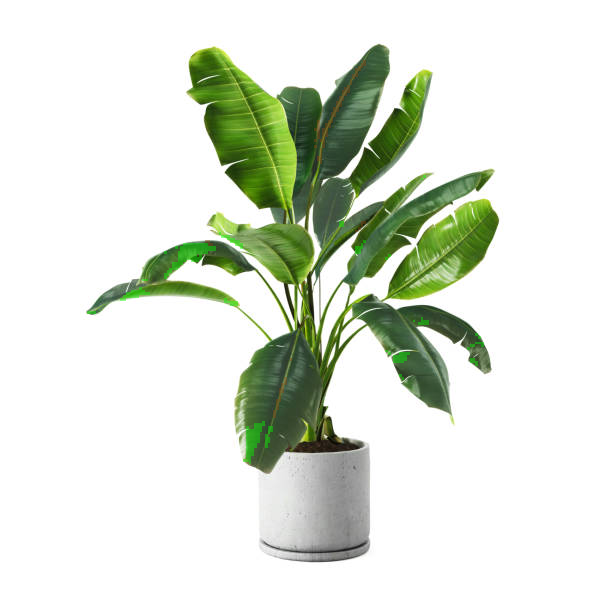
\includegraphics[height=4cm]{../figures/ml_results/attempt1.png}
    \hspace{0.2cm}
    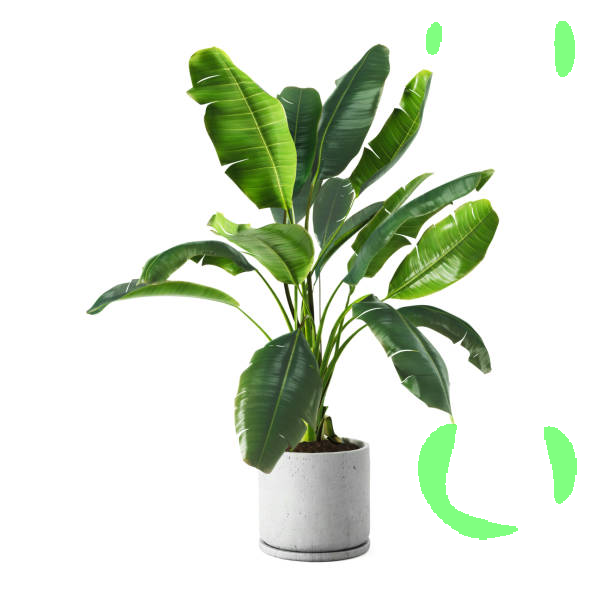
\includegraphics[height=4cm]{../figures/ml_results/attempt2.png}
    \hspace{0.2cm}
    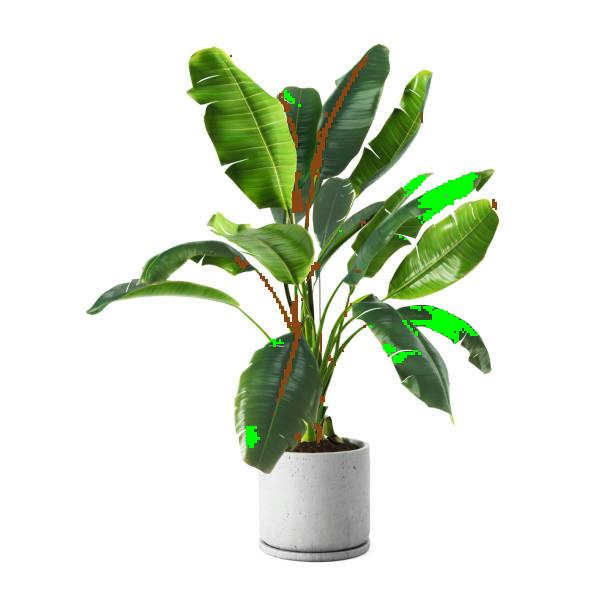
\includegraphics[height=4cm]{../figures/ml_results/attempt3.jpg}
    \caption{Exemplos de tentativas frustradas de detecção automática de caules utilizando diferentes abordagens de machine learning. Fonte: os autores.}
    \label{fig:ml_failed_attempts}
\end{figure}

Dessa forma, a solução final do projeto ficou restrita à detecção e quantificação das folhas, que apresentaram características visuais mais homogêneas e segmentáveis nas imagens disponíveis, permitindo resultados mais confiáveis e reprodutíveis.

\chapter{Resultados}

Nesta seção, apresentamos os principais resultados positivos obtidos com a aplicação desenvolvida para análise do crescimento de plantas via processamento de imagens.

\section{Resultados do Algoritmo}

A aplicação do algoritmo de segmentação proposto resultou em máscaras precisas para a identificação das regiões vegetais nas imagens analisadas, mesmo diante de desafios como variações de iluminação, ruído de fundo e diferenças morfológicas entre as plantas. Os resultados evidenciam que o método é capaz de isolar de forma consistente as áreas verdes, minimizando a inclusão de regiões não pertencentes à planta e preenchendo eventuais falhas na segmentação.

As medidas morfológicas extraídas --- altura, largura e área foliar --- apresentaram boa estabilidade e reprodutibilidade ao longo de diferentes imagens e coleções, permitindo o acompanhamento quantitativo do crescimento das plantas. A sobreposição visual das máscaras segmentadas e das linhas de medição sobre as imagens originais facilita a validação dos resultados, tornando o processo transparente e confiável para o usuário.

\section{Acompanhamento do Crescimento de uma Planta}

A interface gráfica proporciona uma experiência intuitiva e eficiente para o usuário. Por meio dela, é possível organizar fotos em coleções, processar imagens individualmente ou em lote, visualizar resultados detalhados e acompanhar o desenvolvimento das plantas ao longo do tempo. A Figura~\ref{fig:interface-grafica} ilustra a tela principal da aplicação, destacando a organização das coleções.

\begin{figure}[H]
    \centering
    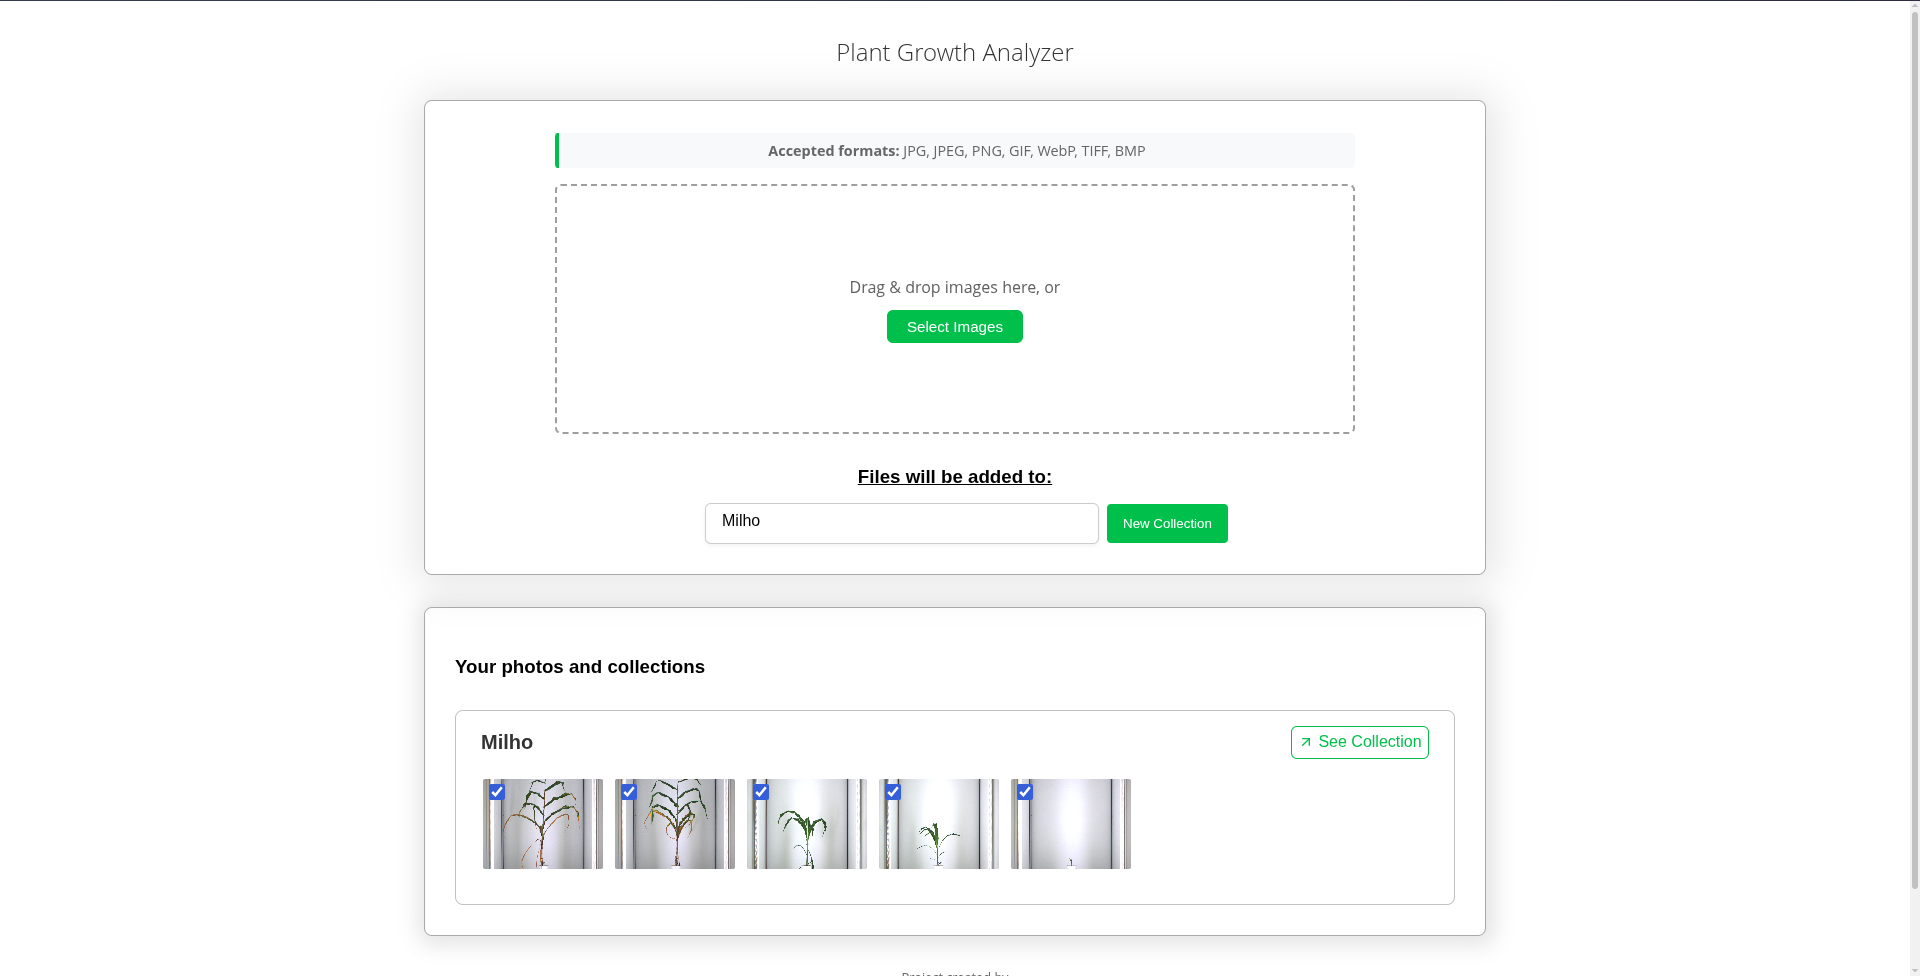
\includegraphics[width=0.9\textwidth]{../figures/screens/interface-grafica.png}
    \caption{Interface gráfica da aplicação. Na imagem, temos a tela inicial do aplicativo, com a opção de enviar imagens para a aplicação. Fonte: os autores.}
    \label{fig:interface-grafica}
\end{figure}

A interface gráfica pode ser dividida em três principais modos de visualização, cada um voltado para uma etapa do fluxo de trabalho do usuário:

\textbf{1. Visualização de Coleções:} A tela inicial da aplicação apresenta as coleções de imagens organizadas pelo usuário. Cada coleção agrupa fotos de uma mesma planta ou experimento ao longo do tempo, facilitando o gerenciamento e a navegação entre diferentes conjuntos de dados. O usuário pode criar, renomear ou excluir coleções, além de adicionar ou remover imagens conforme necessário. A Figura~\ref{fig:colecoes} ilustra essa visualização.

\begin{figure}[H]
    \centering
    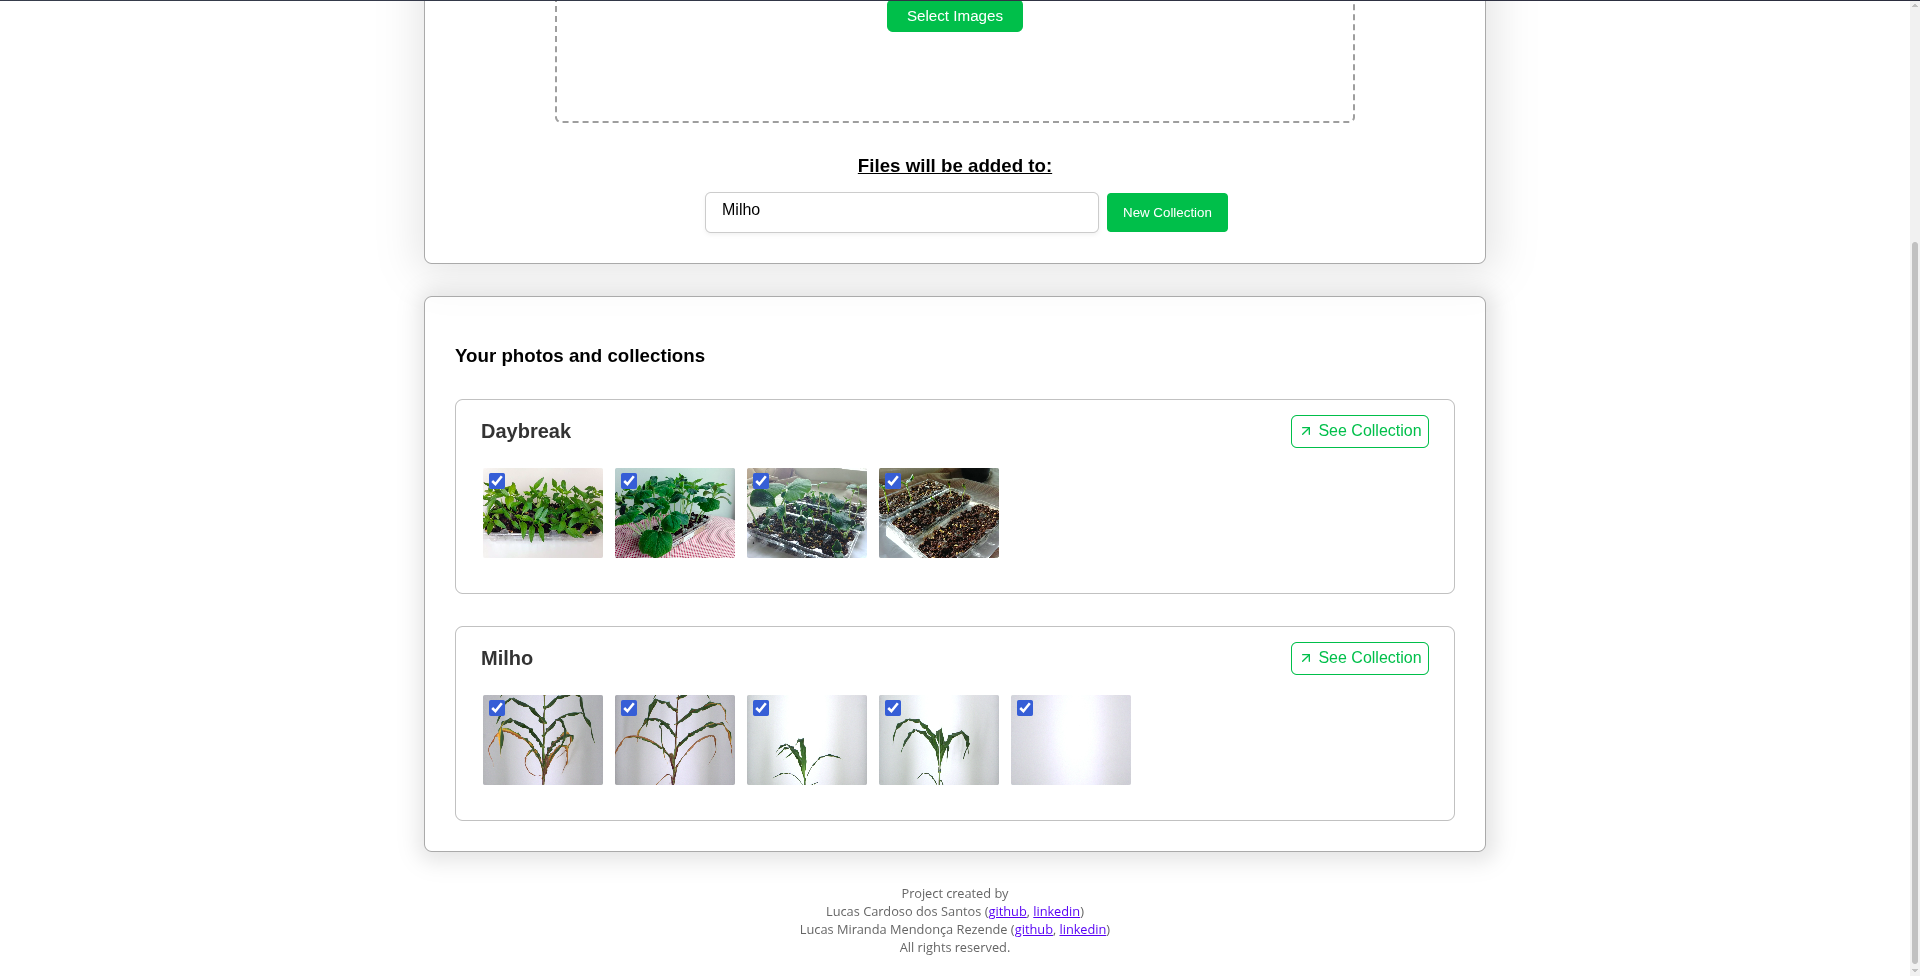
\includegraphics[width=0.9\textwidth]{../figures/screens/colecoes.png}
    \caption{Visualização das coleções de imagens na interface gráfica. Fonte: os autores.}
    \label{fig:colecoes}
\end{figure}

\textbf{2. Visualização dos Resultados de Processamento de uma Imagem:} Ao selecionar uma imagem dentro de uma coleção, o usuário acessa uma tela dedicada à análise individual. Nela, são exibidos lado a lado a foto original e o resultado do processamento: a máscara segmentada sobreposta, as medidas morfológicas extraídas (área, altura e largura) e informações detalhadas sobre a imagem. A Figura~\ref{fig:processamento-individual} mostra um exemplo dessa visualização.

\begin{figure}[H]
    \centering
    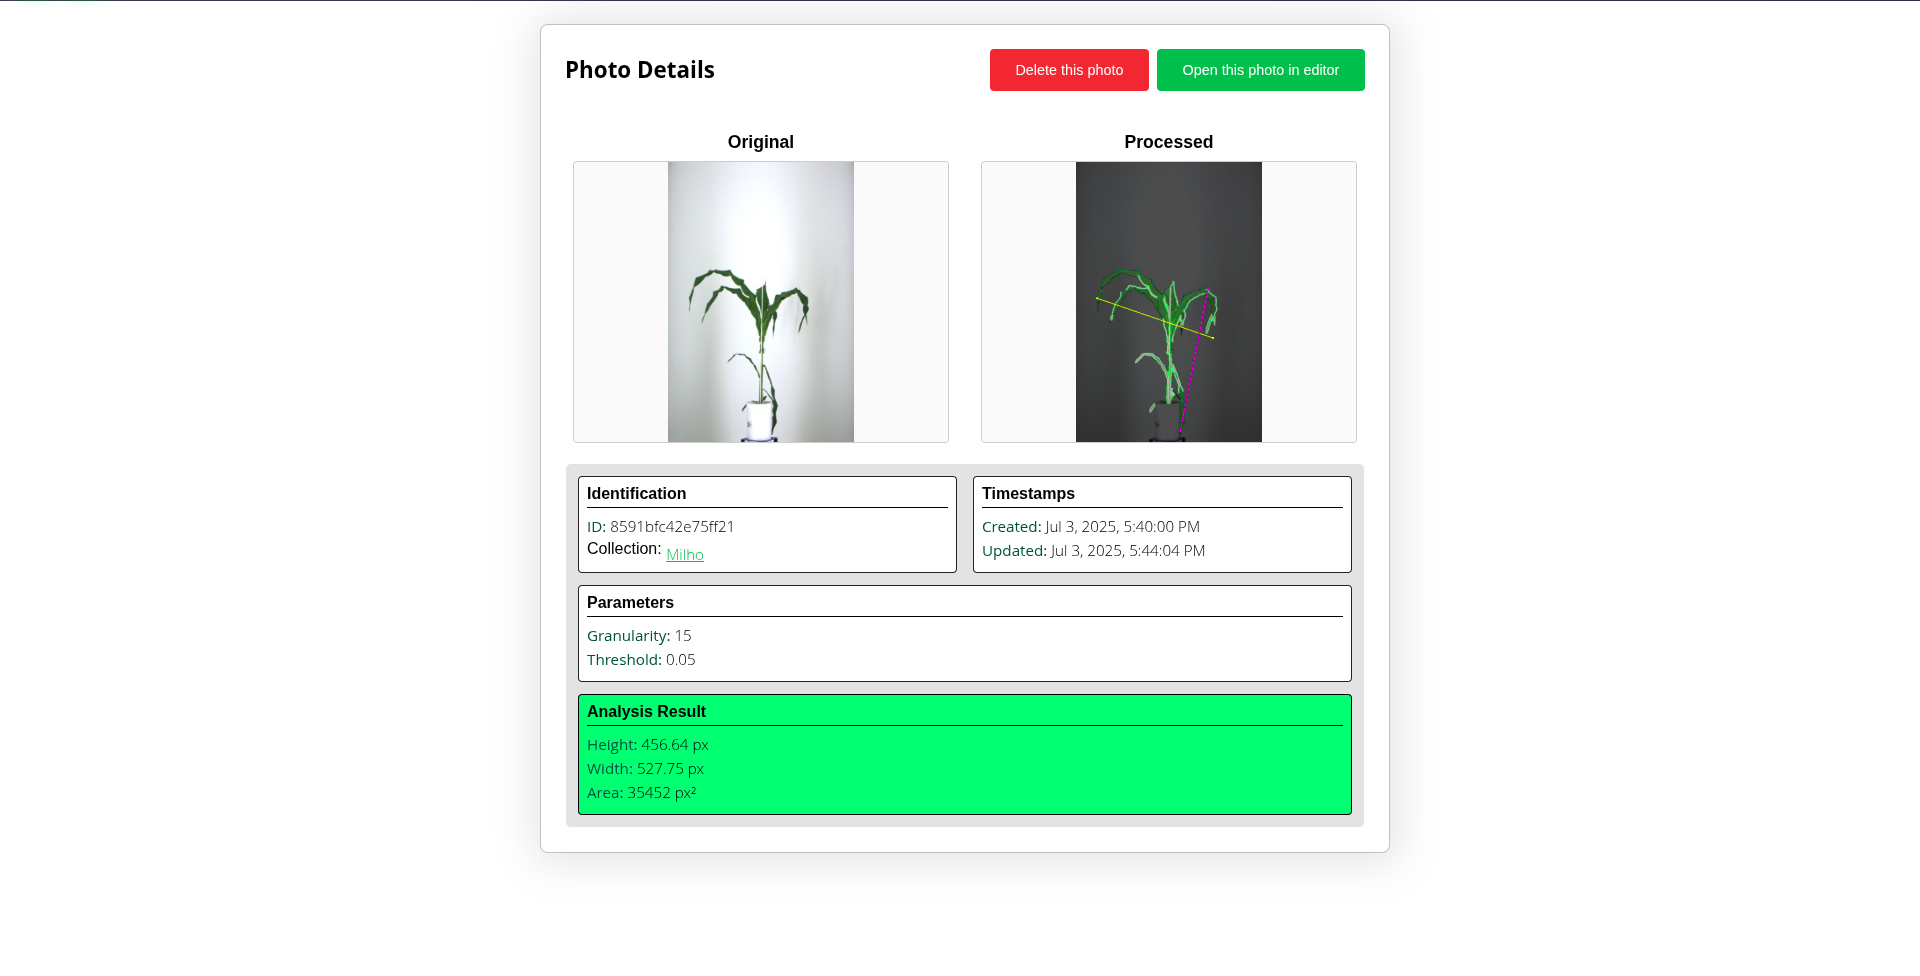
\includegraphics[width=0.9\textwidth]{../figures/screens/processamento-individual.png}
    \caption{Tela de processamento de uma imagem individual, mostrando a visualização dos resultados de segmentação e as medidas extraídas. Fonte: os autores.}
    \label{fig:processamento-individual}
\end{figure}

\textbf{3. Gráficos de Crescimento em uma Coleção:} Para cada coleção, a aplicação gera automaticamente gráficos que mostram a evolução das medidas morfológicas ao longo do tempo, como a área foliar, altura e largura. Esses gráficos permitem ao usuário acompanhar visualmente o desenvolvimento das plantas, identificar tendências e comparar diferentes experimentos. A Figura~\ref{fig:grafico-crescimento} apresenta um exemplo de gráfico de crescimento gerado pela aplicação.

\begin{figure}[H]
    \centering
    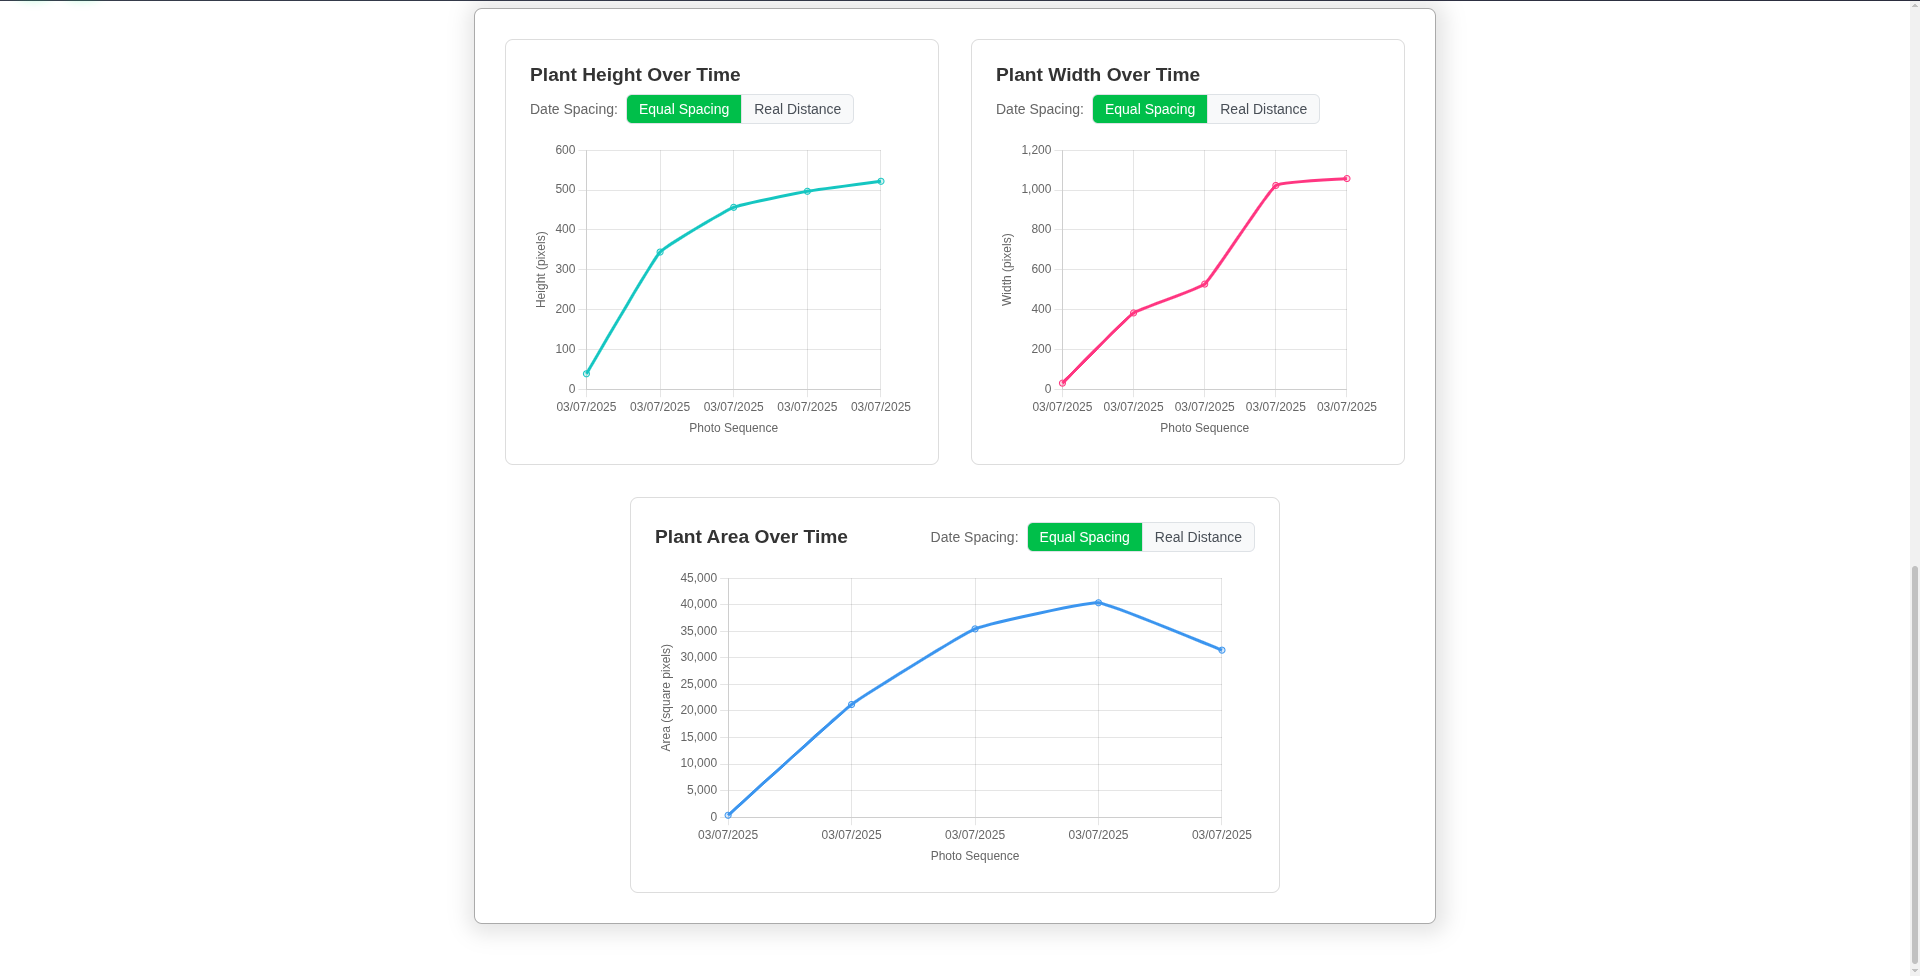
\includegraphics[width=0.9\textwidth]{../figures/screens/grafico-crescimento.png}
    \caption{Gráfico de crescimento mostrando a evolução da área foliar ao longo do tempo em uma coleção. Fonte: os autores.}
    \label{fig:grafico-crescimento}
\end{figure}

Esses resultados demonstram que a solução proposta é eficaz para monitorar o desenvolvimento de plantas de forma automatizada, reprodutível e acessível, atendendo tanto a demandas de pesquisa quanto de ensino ou hobby.





\chapter{Considerações Finais}

O desenvolvimento desta aplicação para análise automatizada do crescimento de plantas demonstra o potencial do processamento de imagens aliado a uma interface gráfica intuitiva para modernizar práticas de monitoramento vegetal. O sistema mostrou-se eficaz na segmentação de folhas e na extração de métricas morfológicas relevantes, permitindo o acompanhamento quantitativo do desenvolvimento das plantas ao longo do tempo.

A flexibilidade e acessibilidade da solução tornam-na adequada tanto para ambientes de pesquisa quanto para uso didático ou por produtores. A organização em coleções, o processamento em lote e a geração automática de gráficos facilitam o gerenciamento de experimentos e a visualização dos resultados.

Apesar dos avanços, algumas limitações persistem, especialmente na detecção do caule, que se mostrou um desafio técnico relevante. Futuras melhorias podem envolver o uso de técnicas mais avançadas de aprendizado de máquina, integração com sensores adicionais ou calibração para conversão de pixels em medidas reais.

Em síntese, a aplicação representa um passo importante para a automação e padronização da análise de crescimento vegetal, contribuindo para decisões mais informadas e para o avanço da Agricultura Inteligente.


\end{document}